\appendix

\section{Cross validation of the ML algorithms}  \label{app:crossval}

To obtain the optimal hyperparameters of our \ac{ML} algorithms, we perform cross-validation across different values of the algorithm parameters. We apply the algorithms to the \ac{O2} data set for different choices of parameters, and we select the combination that gives the highest accuracy.

\subsection{K-Nearest Neighbors}

We utilize the $k$-fold cross validation implemented in scikit-learn~\cite{Pedregosa:2011ork} with $k = 10$ folds, which is a common choice in applied machine learning. As consistency checks, we use different numbers of folds ($k = 4$ and $k=5$) and achieve consistent results in all cases, with an accuracy ranging between 0.9449 and 0.9517. The dataset used for cross-validation is $D=D_R\oplus D_S$.

The \ac{KNN} algorithm's hyperparameters include the number of neighbors ($K$), distance metric, nearest neighbor method, and prediction weight function. Table ~\ref{tab:KNN_crossval_tab} displays many combinations of these parameters and the resulting accuracy following cross-validation. It is worth noting that the choice of hyperparameters has little to no impact on accuracy.

\begin{table}[h]
\begin{tabular}{c|c|c|c|c}
\hline
Neighbors   & Metric & Weights & Algorithm & \multicolumn{1}{|c}{Accuracy} \\ \hline
2                                   & Manhattan                   & Distance                    & BallTree                   &  0.9399                                  \\
2                                   & Euclidean                   & Distance                    & KDTree                   & 0.9392                           \\
2                                   & Manhattan                   & Uniform                    & Auto             &                    0.9359  \\
8                                   & Manhattan                  & Distance                   & BallTree &                    0.9485 \\
8                                   & Euclidean                 & Distance                   & KDTree             &                       0.9477 \\               
8                                   & Manhattan                   & Uniform                   & Auto              &                          0.9468 \\
20                                   & Manhattan                   & Distance                   & BallTree &                  0.9469 \\
20                                   & Euclidean                   & Distance                   & KDTree              &                       0.9459 \\               
20                                   & Manhattan                   & Uniform                   & Auto              &                          0.9437 \\
\hline
\end{tabular}
\caption{Values of the accuracy for different combinations of the hyperparameters. The accuracy in all cases is larger than $0.935$.}
\label{tab:KNN_crossval_tab}
\end{table}

Figure~\ref{fig:crossvalKNN} illustrates the accuracy dependence on different hyperparameter options while keeping the algorithm used to compute nearest neighbors, the BallTree, constant.

\begin{figure*}%[h]
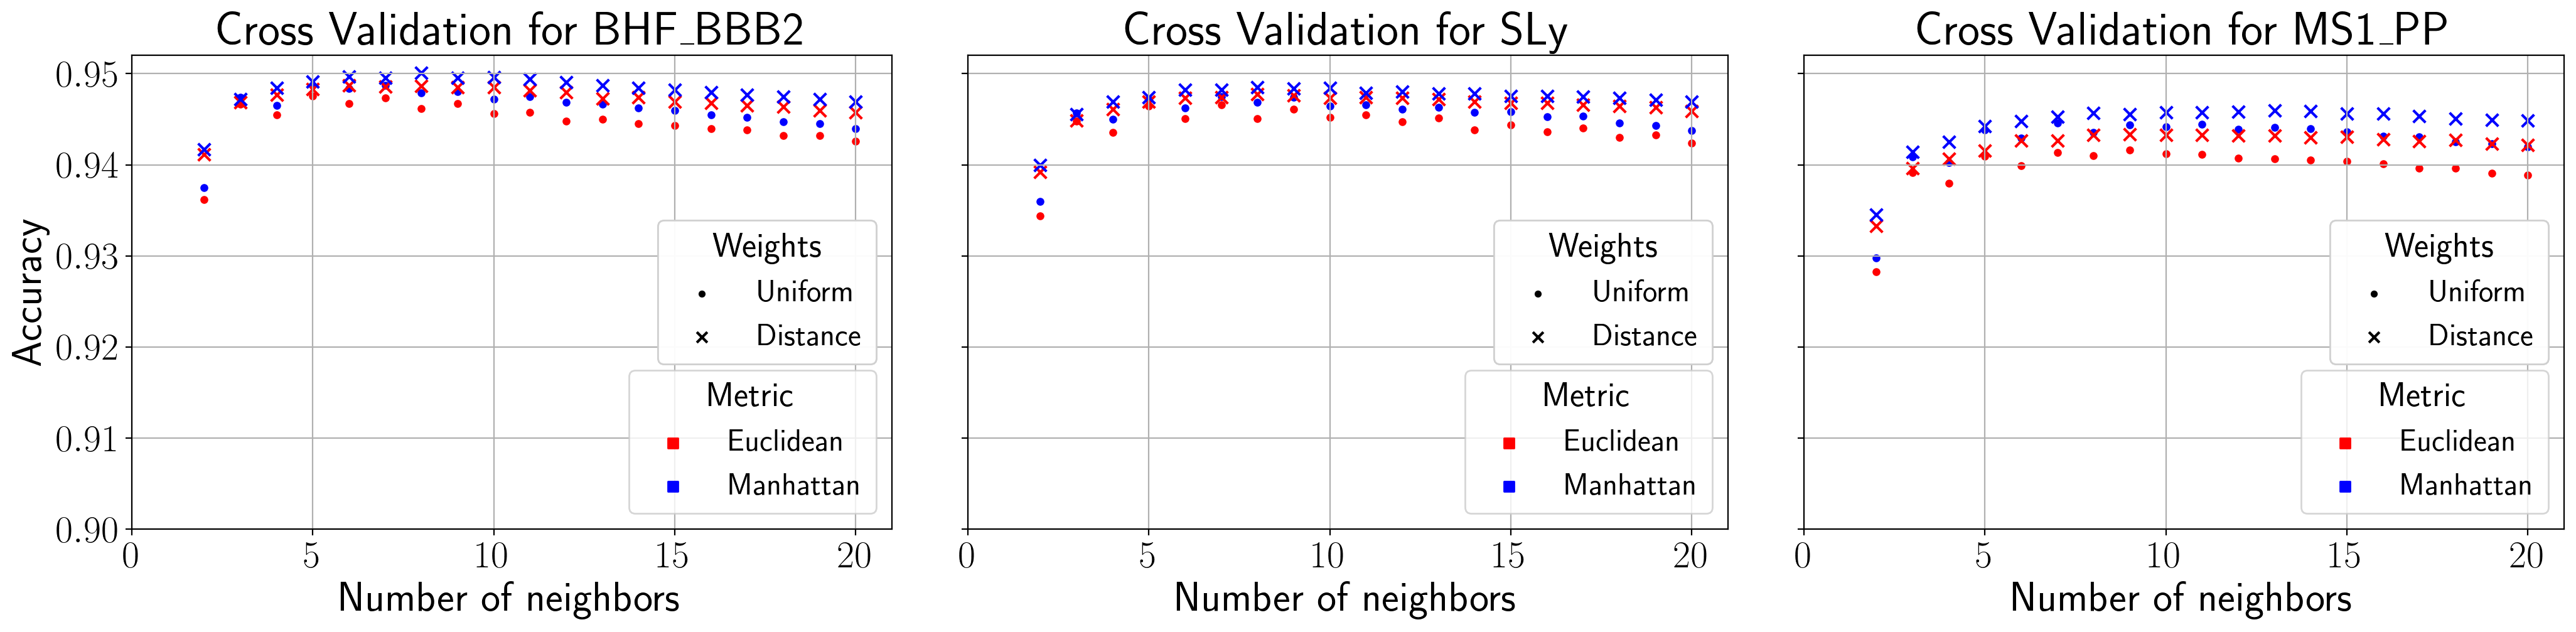
\includegraphics[width=\linewidth]{cross_val_KNN}
\caption{Accuracy of the \ac{KNN} algorithm as a function of the number of neighbors. The color red (blue) denotes the Euclidean (Manhattan) metric, and the dots (crosses) denote uniform (distance) weights. The BallTree algorithm is used to find the nearest neighbors. The accuracy does not significantly change when more than 5 neighbors are considered.}
\label{fig:crossvalKNN}
\end{figure*}

The ideal hyperparameters are the same for all state equations, with the exception of the number of neighbors, which varies between 6 and 12.  We use the Bayes factors described in~\cite{Ghosh:2021eqv} to marginalize over all state equations. The marginalized optimal number of neighbors is 8. However, as illustrated in Fig.~\ref{fig:crossvalKNN}, there is no significant change in accuracy when a higher number of neighbors is used. Table~\ref{tab:KNN_opt_params} shows the fixed hyperparameters used in our KNN implementation.

\begin{table}[h]
\begin{tabular}{c|c|c|c}
\hline
Nº of neighbors   & Metric & Weights & Algorithm  \\ \hline
8  & Manhattan  & Distance & BallTree \\ 
\hline
\end{tabular}
\caption{Optimal hyperparameters for the \ac{KNN} algorithm. These are the values we use to train and test the algorithm, as well as to calculate Bayesian probabilities.} \label{tab:KNN_opt_params}
\end{table}


\subsection{Random Forest}

To apply cross-validation to the \ac{RF} algorithm, we use the training ($D_R$) and testing ($D_S$) data sets presented in Section~\ref{probability}. We choose possible values for the various hyperparameters and compare the accuracy of the generated forests. Unlike \ac{KNN}, \ac{RF} does not apply the $k$-fold cross-validation procedure. This is because the implementation of \ac{RF} we employ admits the bootstrap technique in the training. Each tree in the forest accesses a random subset of the training data, thus achieving the same effect.

We investigate the effect on accuracy by varying the number of trees in the forest, the method used to compute the information gain after each node split (gini or entropy), the maximum number of features considered in each node (the square root of the total number of features, or all of them), and the maximum depth that the trees can reach. For tree depth, we explore two options: None, which consists of allowing the trees to grow until data points are isolated at the leaves, and 15. We chose this figure since it is half the average depth obtained with the None option.

We use the Bayes factors to marginalize on the configurations that lead to the highest score for each \ac{EOS}. We conclude that for all \ac{EOS}, we should employ 81.017 trees, the ``entropy'' criterion, the square root of the number of features at split, and a depth equal to 15.


\begin{table}[h]
\begin{tabular}{|l|c|}
\hline
Trees& 81.02 \\
Criteria (0-gini, 1-entropy)& 0.9577 \\
Features (0-sqrt, 1-All)& 0.3902  \\
Depth (0-15 depth, 1-None)& 0.0000 \\ \hline
\end{tabular}
\caption{Optimal hyperparameters for the \ac{RF} algorithm. \label{tab:RF_cross_params}}
\end{table}

Table \ref{tab:RF_cross_params} displays the results of hyperparameter marginalization over the \ac{EOS}. For any \ac{EOS}, regardless of other hyperparameters, a depth of 15 yields higher accuracy. The "entropy" criterion is adopted for practically every \ac{EOS}, whereas the number of features to consider is more tightly restricted.

Figure~\ref{fig:crossvalRF} displays the accuracies obtained during cross-validation, with the depth fixed to 15. It is worth noting that using more trees results in higher scores. Nonetheless, the goal of making this method run in low latency favors smaller files (with less tree information) that can be loaded rapidly. Therefore, given the difference in accuracy and size of the trained models, we limit ourselves to 50 trees.

\begin{figure*}%[h]
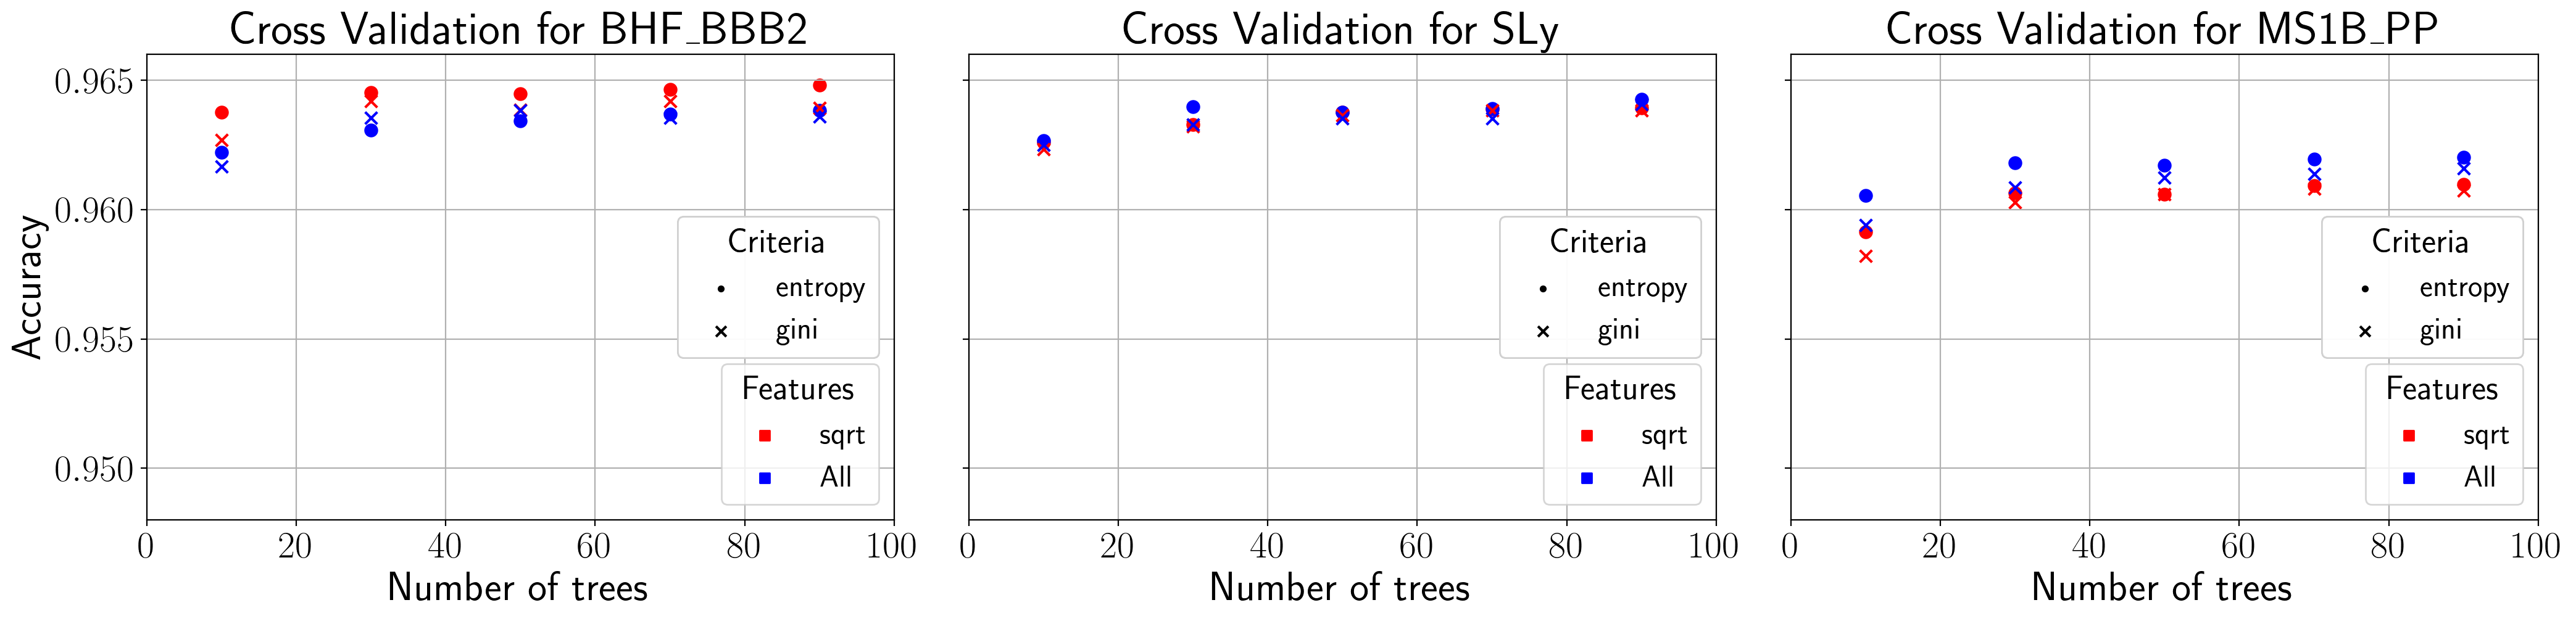
\includegraphics[width=\linewidth]{cross_val_RF}
\caption{Accuracy of the \ac{RF} algorithm as a function of the number of trees.  The color red (blue) denotes ``sqrt'' (``all'') features, while the dots (crosses) denote ``entropy'' (``gini'') criteria. The depth of the trees is set at 15. All cases have an accuracy range of 0.960 to 0.965.}
\label{fig:crossvalRF}
\end{figure*}

\section{Comparison between our algorithms and the current LVK implementation}  \label{app:comparison}

To compare the existing \ac{LVK} implementation of \ac{KNN}~\cite{Chatterjee:2019avs} with our multi-label \ac{KNN} and \ac{RF} schemes, we show the \ac{ROC} curves for the three methods in Fig.~\ref{fig:rocO2_all}. To provide a fair comparison, we trained the LVK's \ac{KNN} classifier for two cases (\hasns and \hasrem) separately, resulting in a binary label method. In this instance, we use the hyperparameters that are currently configured in the low-latency implementation: $K = 2n + 1 = 11$ neighbors (where $n$ is the number of features), and neighbor weighting by the inverse of distance. Both classifiers were trained using the same 70\% of the \ac{O2} dataset (the $D_R$ subset)\footnote{The current LVK implementation trains the \ac{KNN} algorithm on the entire dataset $D$. This leaves no events to test. Therefore, to ensure a fair comparison, we use a 70\%-30\% split.}. The ROC curve below was generated using the remaining 30\% of the dataset (the $D_S$ subset). The multi-label RF method achieves a high \ac{TPR} across the entire range of \ac{FPR} for both \hasns\ and \hasrem. Both multi-label and binary-label \ac{KNN} methods perform similarly. These \ac{ROC} curve comparisons were done in the same way as in Figures~\ref{fig:rocO2_KNN} and~\ref{fig:rocO2_RF} before defining Bayesian probabilities, as they were generated from the testing set.

\begin{figure*}%[h]
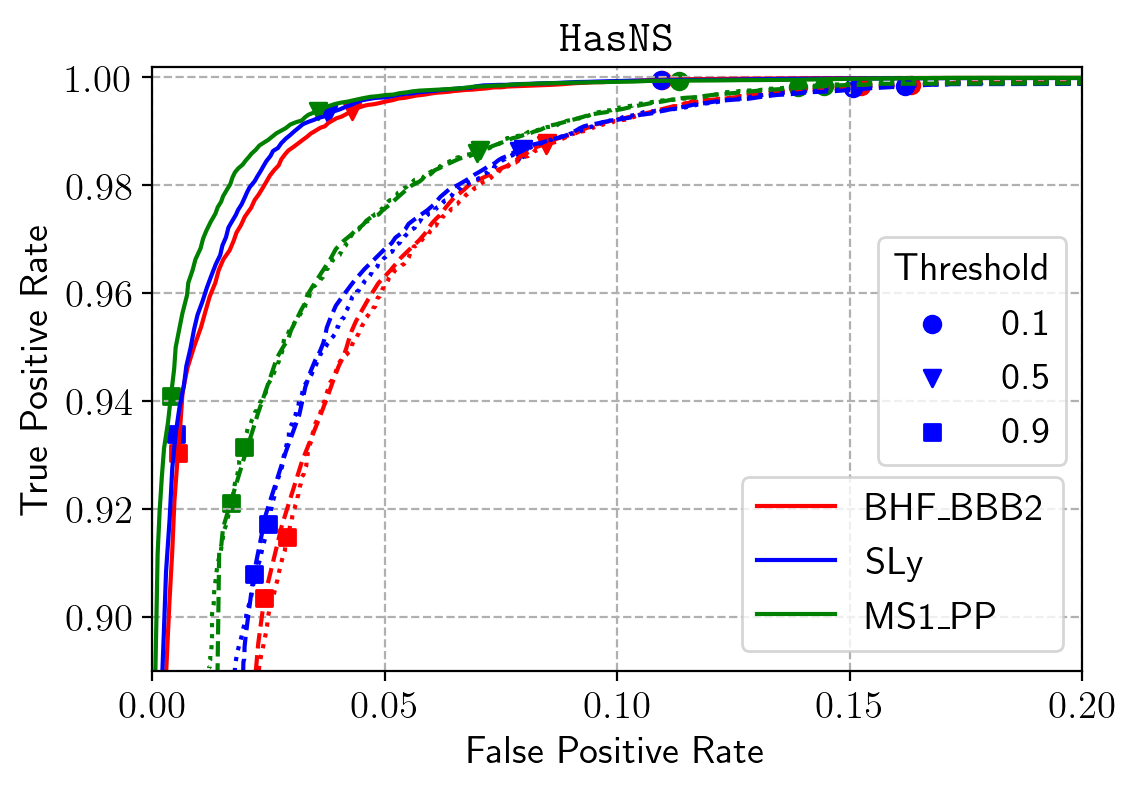
\includegraphics[width=0.47\linewidth]{ROC_O2testing_all_impl-NS}
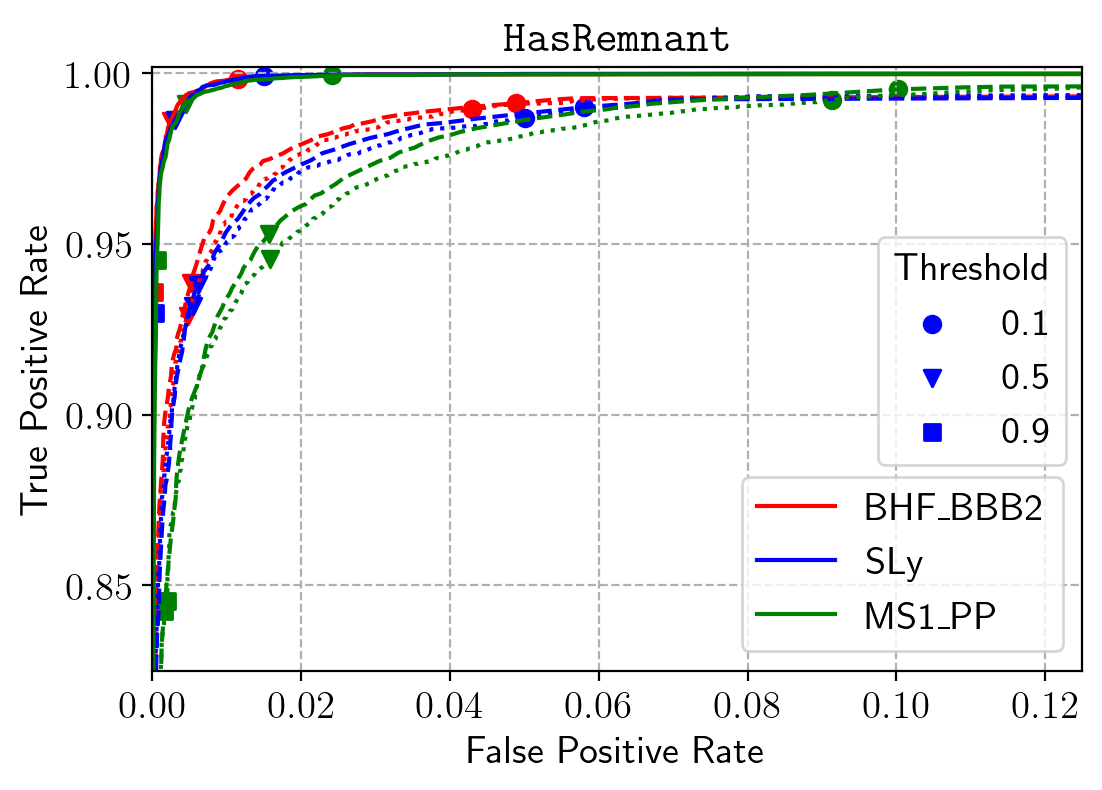
\includegraphics[width=0.45\linewidth]{ROC_O2testing_all_impl-REM}
\caption{\ac{ROC} curves derived from the \ac{O2} testing data set $D_S$ for the \ac{RF} classifier (solid lines), the \ac{KNN} implementation presented in this paper (dashed lines), and the \ac{KNN} approach currently used by the \ac{LVK} Collaborations (dotted lines). The curves for {\tt BHF\_BBB2}, {\tt MS1\_PP}, and {\tt SLy} are colored red, green, and blue, respectively. The circle, triangle, and square marks represent score thresholds of 0.1, 0.5, and 0.9, respectively.}
\label{fig:rocO2_all}
\end{figure*}




